\subsection{Mitocondria Striatum}
For the Mitocondria Striatum set, CNN are employed to solve a segmentation problem. Every pixel is classified as being part of the mitocondria or not. A patch of 51x51 surrounding the pixel is extracted from the image and fed as input to a CNN which acts as a binary classifier. For determining the parameters of the CNN we used a set of
100.000 samples for training and 20.000 for validation (containing half positive and half negative samples). After determining the best setup, the network was trained on a larger set of 1 milion samples for training and 200.000 for validation.

The final test data represented a 3D image volume consisting of 318 slices of size 400x661. Thus, one frame contains 264.400 datasamples that are fed as test input for the CNN, while all frames contain 97 million datasamples.

The best setup obtained using the small training and validation set is the one presented in Table\ref{fig:CNN3} NonSep. This gave us a VOC error on the first frame of 77.2. We then trained this net on the big set and obtained an error of 74. We notice that this is not comparable with state of the art methods which achieve results higher than 79 VOC or that use 3D information. The goal of this
is to see if we can obtain a speedup by using separable filters.
\begin{table}
\centering
\begin{tabular}{@{}rlll@{}}\toprule
Layer & Type & Maps and neurons& Kernel size \\ \midrule
0 & input & 1 map of 51x51 &\\
1& convolutional & 10 maps of 46x46 & 6x6\\
2 & max pooling & 10 maps of 23x23 &  \\
3 & convolutional & 20 maps of 18x18& 6x6 \\
4 & max pooling & 20 maps of 9x9& \\ 
3 & convolutional & 50 maps of 4x4& 6x6 \\
4 & max pooling & 50 maps of 2x2& \\ 
5 & fully conntected& 100 & \\
6 & fully conntected & 2 neurons & \\ \bottomrule
\end{tabular}
\caption{CNN Model for Mitocondria dataset}
\label{fig:CNN3}
\end{table}
Example of the weights learned in the first convolutional layer are shown in Fig[ref] and of output on one frame produced by the CNN. 
\begin{table}
\centering
\begin{tabular}{@{}rllll@{}}\toprule
 &&Conv L1& Conv L2 & Conv L3\\ \midrule
NonSep &Kernel Size & 10 maps 6x6& 20 maps 6x6 & 50 maps 6x6\\
&Speedup rank& $\leq$16.36 & $\leq$22.5 & $\leq$29.03\\
&Theoretical rank & 16.4 & $\leq$36 & 36 \\ 
&time & 8.1 & 26.8 & 18.4 \\ \midrule
Separable& rank & - & 20 & 36 \\ 
& time& - & 20.1 & 17.6\\ \midrule
\end{tabular}
\caption{Results for CNN Mitocondria}
\label{fig:CNN3}
\end{table}
\begin{figure}[h!]
  \centering
  \begin{subfigure}[b]{0.40\textwidth}
   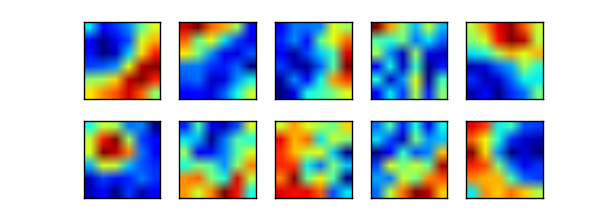
\includegraphics[width=\textwidth]{images/filters.png}
    \caption{Weights learned in the 1st layer}
  \end{subfigure}
  \begin{subfigure}[b]{0.40\textwidth}
    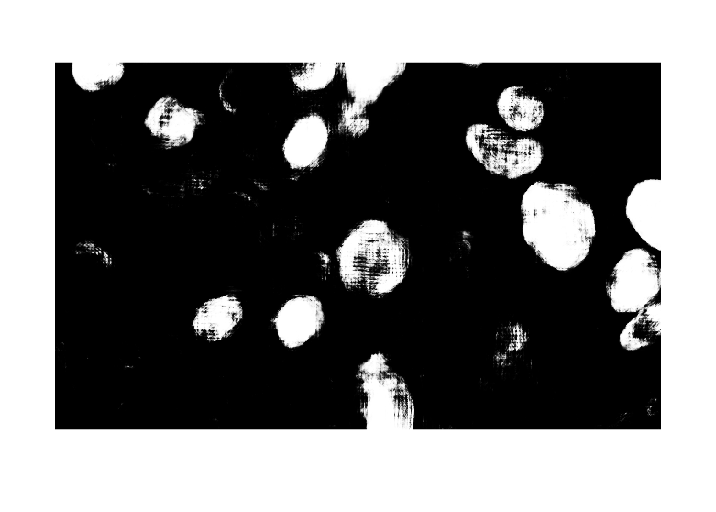
\includegraphics[width=\textwidth]{images/frame1.png}
    \caption{CNN output frame, not thresholded}
  \end{subfigure}
    \begin{subfigure}[b]{0.40\textwidth}
   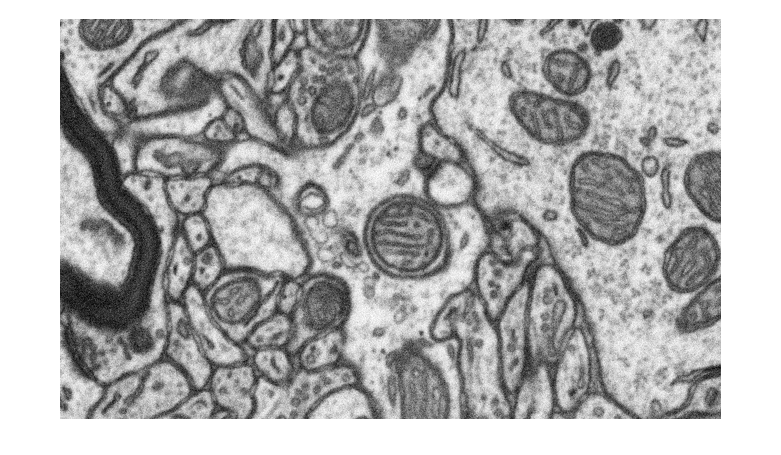
\includegraphics[width=\textwidth]{images/GT_truth.png}
    \caption{CNN input frame}
  \end{subfigure}
  \begin{subfigure}[b]{0.40\textwidth}
    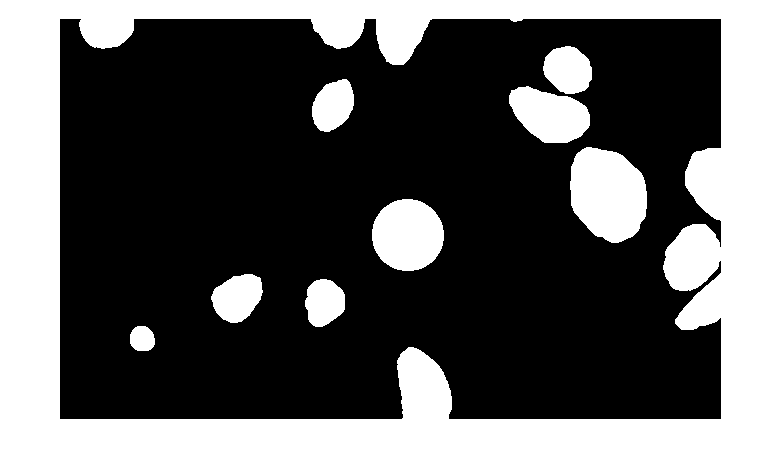
\includegraphics[width=\textwidth]{images/GTframe1.png}
    \caption{Groundtruth frame}
  \end{subfigure}
  \caption{Input and output example of CNN for mitocondria dataset. Fig a) shows that the filters are mostly edges and circles detectors which constitute basic building blocks for the interior of the mitocondria.
  Comparing b), c) and d) we notice the 'noisy' nature of the CNN output for pixel classification. Preprocessing the final output b) using a median filter would likely improve the results.}
  \label{fig:mitocondria}
\end{figure}
We keep conv L1 fixed and approximate conv L2 and L3 with rank 20 and 36 respectively. For the 3rd layer no significant change in performance is observed, while for layer 2 we notice a small speedup from roughly 26 to 20 ms. Since the fit of the two layers was very good (99.9) there was no drop in classification performance.

Fig \ref{fig:mitocondria} shows an example of the CNN input and output and the type of filters that it learns. 
\subsection{Pretrained ImageNet CNN}
As initial step for future work, we investigated how well the separable filters approximation works for large filter banks, like the ones present in deep CNN models used in ImageNet. The network setup in Table\ref{fig:imagenet} is the reference net (without the split to be run on two GPUs) from the initial breakthrough of CNNs in ImageNet challenge by \cite{Krizhevsky_imagenetclassification}. We did not train the network ourselves, but experimented with a pretrained model by \cite{chatfield14return}.

Fig\ref{fig:user_artiststribution} shows the fit of the approximation (mean and variance) with varying rank for the first four convolutional layers.

We notice that the approximation works very well for Conv L1 (64 filters of size 11x11) which have a theoretical rank of almost 50 and we obtain a theoretical speedup if we use a rank smaller than $\frac{64\times 11\times 11}{64 + 11 + 11} = 90$. Thus, we expect almost a 2-fold speedup for the first convolutional layer without loss in performance. If we approximate filters of larger size the speedup is in general bigger. 

Conv L2 has a theoretical rank of 25 and we obtain a speedup if we use a rank $\leq$ 24. We notice that if we try to approximate the initial filters with a rank smaller than 20 the algorithm does not always converge like in all previous experiments. This was also the case for ranks larger than 30, for which we needed to rerun the algorithm with diffferent random intialization until it converged.

Conv L3 and L4 have a theoretical rank of 9 and to obtain a speedup we need to use a rank $\leq8.7$. For a 2-fold speedup, we would need to approximate conv L3 and L4 with rank 4, for which the fit is 86.

\begin{table}[h!]
\centering
\begin{tabular}{@{}rllllllll@{}}\toprule
Arch & conv1 & conv2&  conv3& conv4& conv5& full6& full7 &full8 \\ \midrule
CNN-F & 64x11x11 & 256x5x5& 256x3x3&256x3x3&256x3x3&4096&4096&1000\\
\end{tabular}
\caption{Pre trained ImageNet model  \cite{chatfield14return}.}
\label{fig:imagenet}
\end{table}

%\begin{figure}[!htb]
%  \centering
%   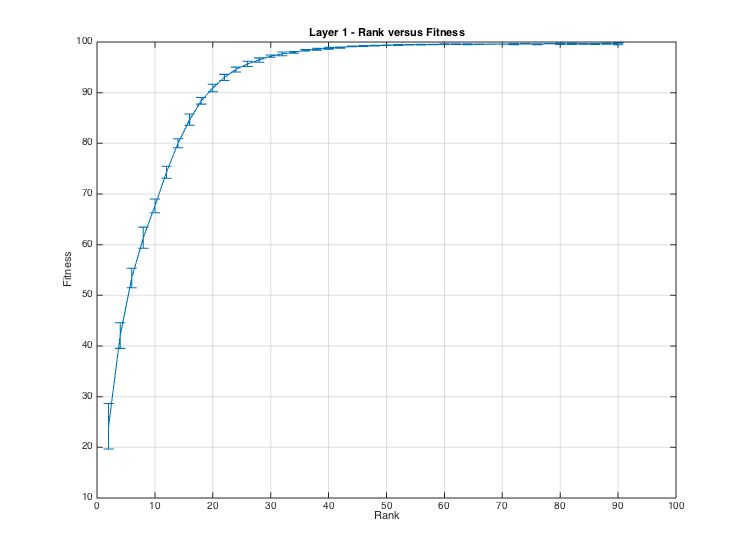
\includegraphics[width=\textwidth]{images/Layer1ImageNet.png}
%    \caption{Conv Layer 1}
%  \end{figure}
%\begin{figure}[!htb]
%  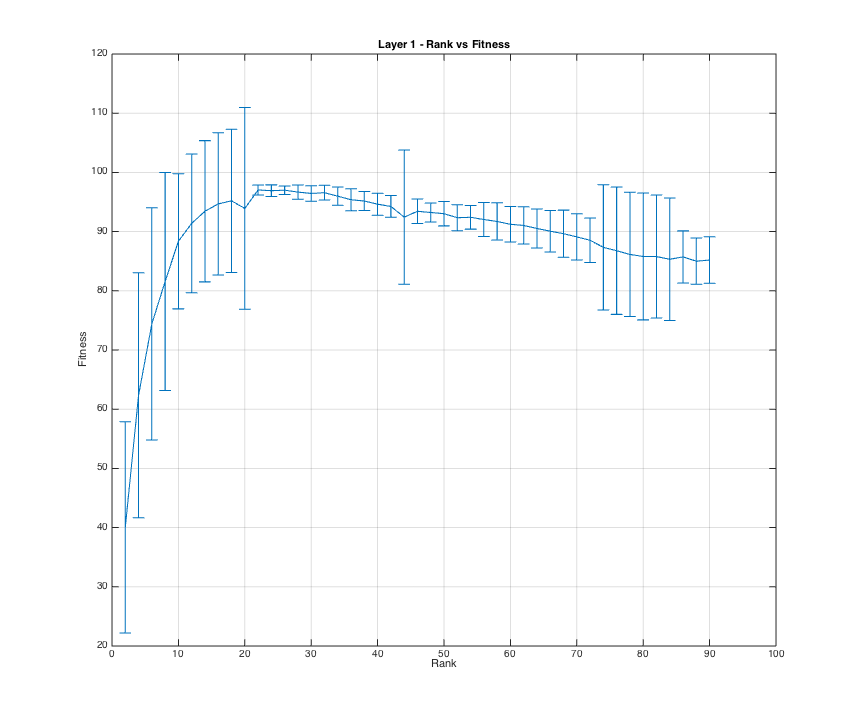
\includegraphics[width=\textwidth]{images/Layer2ImageNet.png}
%    \caption{Conv Layer 2}
%  \end{figure}
%  \begin{figure}[h]{0.40\textwidth}
%   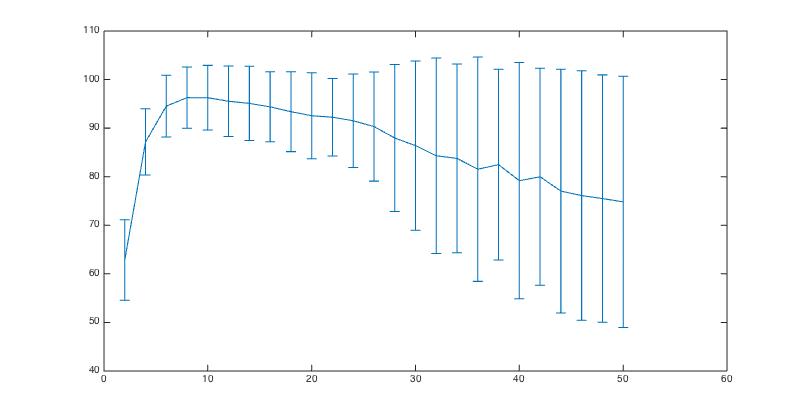
\includegraphics[width=\textwidth]{images/Layer3ImageNet.png}
%    \caption{Conv Layer 3}
%  \end{figure}
%  \begin{figure}[h]{0.40\textwidth}
%    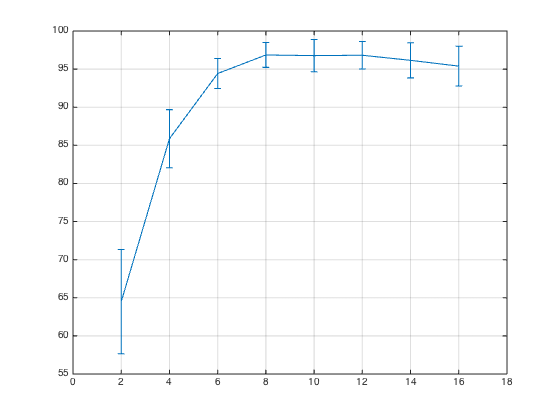
\includegraphics[width=\textwidth]{images/Layer4ImageNet.png}
%    \caption{Conv Layer 4}
%  \end{figure}

\begin{figure}[!htb]
  \centering
  \begin{subfigure}[h]{0.40\textwidth}
   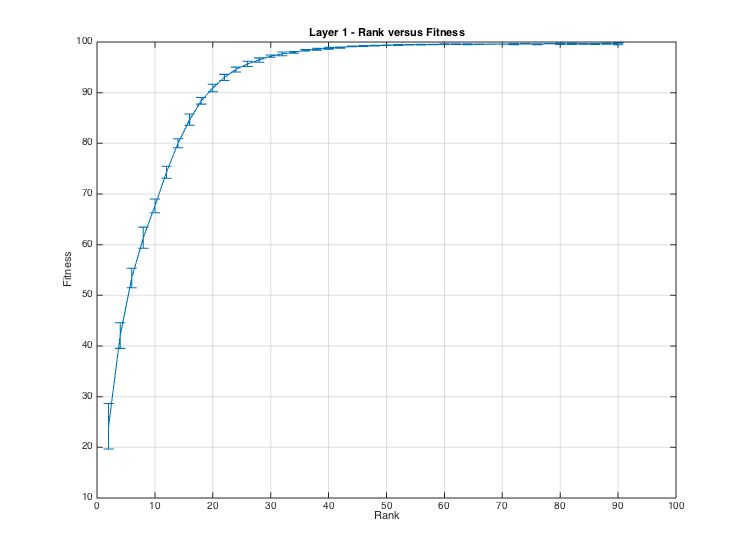
\includegraphics[width=\textwidth]{images/Layer1ImageNet.png}
    \caption{Conv Layer 1}
  \end{subfigure}
  \begin{subfigure}[h]{0.40\textwidth}
    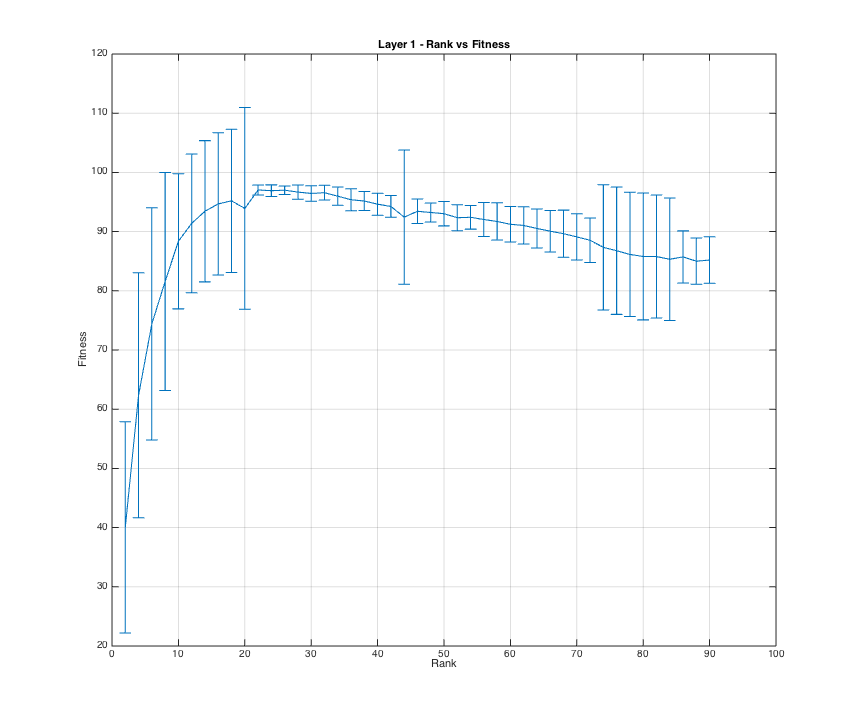
\includegraphics[width=\textwidth]{images/Layer2ImageNet.png}
    \caption{Conv Layer 2}
  \end{subfigure}
  \begin{subfigure}[h]{0.40\textwidth}
   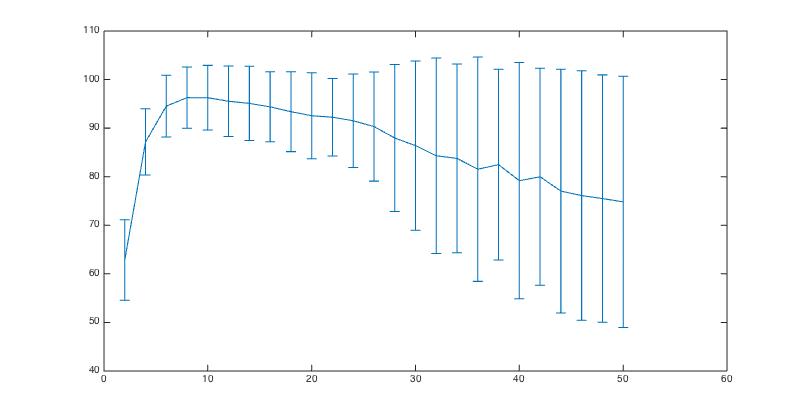
\includegraphics[width=\textwidth]{images/Layer3ImageNet.png}
    \caption{Conv Layer 3}
  \end{subfigure}
  \begin{subfigure}[h]{0.40\textwidth}
    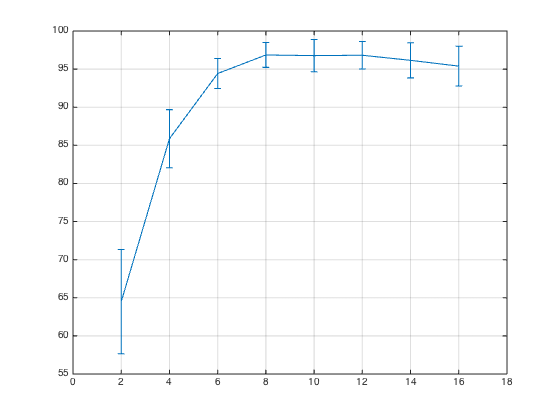
\includegraphics[width=\textwidth]{images/Layer4ImageNet.png}
    \caption{Conv Layer 4}
  \end{subfigure}
  \caption{Rank versus Fit for Conv Layers of ImageNet model. Conv L1 can have a theoretical 2-fold speedup while the approximation is almost perfect (rank aprox. 45 with fit 99.9). For the following layers, the optimization algorithm starts to struggle and needs to be rerun multiple times. For a similar 2-fold speedup per layer, we would need to use a rank for which the fit is less than 90.}
  \label{fig:user_artiststribution}
\end{figure}
